% generated by Plantuml 1.2018.13      
\definecolor{plantucolor0000}{RGB}{254,254,206}
\definecolor{plantucolor0001}{RGB}{168,0,54}
\definecolor{plantucolor0002}{RGB}{173,209,178}
\definecolor{plantucolor0003}{RGB}{0,0,0}
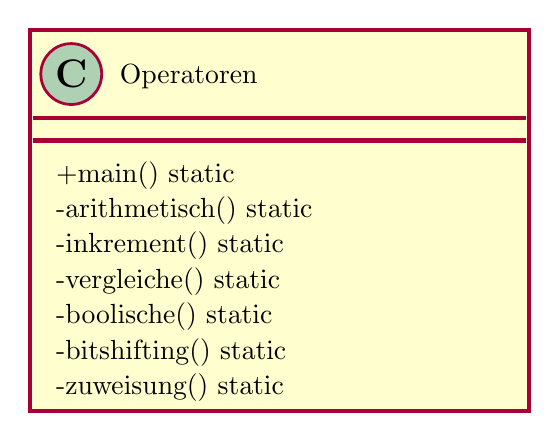
\begin{tikzpicture}[yscale=-1
,pstyle2/.style={color=plantucolor0001,line width=1.5pt}
]
\draw[color=plantucolor0001,fill=plantucolor0000,line width=1.5pt] (6pt,8pt) rectangle (186.4063pt,145.6328pt);
\draw[color=plantucolor0001,fill=plantucolor0002,line width=1.0pt] (21pt,24pt) ellipse (11pt and 11pt);
\node at (21pt,24pt)[]{\textbf{\Large C}};
\node at (35pt,17.0156pt)[below right,color=black]{Operatoren};
\draw[pstyle2] (7pt,40pt) -- (185.4063pt,40pt);
\draw[pstyle2] (7pt,48pt) -- (185.4063pt,48pt);
\node at (12pt,52pt)[below right,color=black]{+main() static};
\node at (12pt,64.8047pt)[below right,color=black]{-arithmetisch() static};
\node at (12pt,77.6094pt)[below right,color=black]{-inkrement() static};
\node at (12pt,90.4141pt)[below right,color=black]{-vergleiche() static};
\node at (12pt,103.2188pt)[below right,color=black]{-boolische() static};
\node at (12pt,116.0234pt)[below right,color=black]{-bitshifting() static};
\node at (12pt,128.8281pt)[below right,color=black]{-zuweisung() static};
\end{tikzpicture}
